\documentclass[11pt]{article}
\usepackage{anysize}
\marginsize{2.75cm}{2.75cm}{1.75cm}{1.75cm}
%\marginsize{left}{right}{top}{bottom}
\usepackage{amsmath}
\usepackage{dsfont}
%\usepackage[dvips]{graphicx}
\usepackage{graphicx}
\usepackage{lscape}
	
\usepackage{pdflscape}
\usepackage{array}
\usepackage{rotating,capt-of,varwidth}
\usepackage{longtable}
\usepackage{setspace}
%\usepackage{harvard}
\usepackage{color}
\usepackage{tabularx}
\usepackage{booktabs}
\usepackage{multirow}
\usepackage{subfigure}
\usepackage[figuresright]{rotfloat}
%\usepackage{epstopdf}
\usepackage{natbib}
\usepackage[justification=centering]{caption}


\pagestyle{plain}

\bibliographystyle{dcu}
%\citationstyle{dcu}

\parindent0em
\parskip2.0ex plus0.5ex minus0.2ex

\renewcommand{\thesubfigure}{\thefigure.\arabic{subfigure}}

\newcommand{\maketableline}{\noalign{\smallskip}\midrule\noalign{\smallskip}}
\newcommand{\maketabletopline}{\noalign{\smallskip}\toprule\noalign{\smallskip}}
\newcommand{\maketablebottomline}{\noalign{\smallskip}\bottomrule\noalign{\smallskip}}
\newcommand{\mc}{\mathcal}
\newcommand{\sumlow}{\sum\nolimits}
\newcommand{\fref}[1]{Figure \ref{#1}}
\newcommand{\fsref}[2]{Figures \ref{#1} to \ref{#2}}
\newcommand{\fandref}[2]{Figures \ref{#1} and \ref{#2}}
\newcommand{\eref}[1]{Equation (\ref{#1})}
\newcommand{\esref}[2]{Equations (\ref{#1}) to (\ref{#2})}
\newcommand{\eandref}[2]{Equations (\ref{#1}) and (\ref{#2})}
\newcommand{\tref}[1]{Table \ref{#1}}
\newcommand{\tsref}[2]{Tables \ref{#1} to \ref{#2}}
\newcommand{\tandref}[2]{Tables \ref{#1} and \ref{#2}}
\newcommand{\sref}[1]{Section \ref{#1}}
\newcommand{\sandref}[2]{Sections \ref{#1} and \ref{#2}}
\newcommand{\ssref}[2]{Sections \ref{#1} to \ref{#2}}
\newcommand{\aref}[1]{Appendix \ref{#1}}
\renewcommand{\footnoterule}{\rule{6cm}{0.2pt}\vspace{3pt}}
\newcommand{\mb}[1]{\text{\boldmath$#1$}}
\newcommand{\tc}{\textcolor}

\linespread{1.2}
\begin{document}

\section{Data and descriptive statistics}

The aim of our research project is to estimate the impact of foreign direct investment (FDI) on labor market outcomes. More specifically, we analyze the effect of FDI on employment and wages. We use firm-level data for the years 2015 to 2017. In 2016, some of the firms receive FDI. The receipt of FDI is referred to as treatment in the following. Table \ref{sumstat} shows summary statistics for the main variables included in our dataset, both for 2015 -- i.e. our pre-treatment period -- and 2017 -- i.e. the post-treatment  period. We have information on wages, employment, total factor productivity (TFP), debt, export intensity as well as a dummy variable indicating whether a firm engages in research and development activities. In total, 11,323 firms are included in our dataset. On average, wages decreased from 2015 to 2017, while TFP, employment, export intensity, and the share of firms engageing in R\&D  increased. We do not have information on debt in 2017.


\begin{table}[htbp]\centering \caption{Summary statistics\label{sumstat}}
{
\def\sym#1{\ifmmode^{#1}\else\(^{#1}\)\fi}
\begin{tabular}{l*{1}{ccccc}}
\hline\hline
                    &\multicolumn{5}{c}{}                                            \\
                    &        Mean&   Std. Dev.&        Min.&        Max.&        Obs.\\
\hline
Wages in 2015 (logs)&       7.333&       3.839&      -7.332&      22.432&       11323\\
Total factor productivity in 2015&       3.041&       2.047&      -5.359&      11.357&       11323\\
Employment in 2015 (logs)&       4.411&       3.040&      -6.229&      15.993&       11323\\
Debt in 2015 (logs) &       0.504&       0.353&      -0.200&       1.300&       11323\\
Export intensity in 2015&       0.159&       0.080&       0.010&       0.483&       11323\\
RD in 2015 (dummy)  &       0.121&       0.326&       0.000&       1.000&       11323\\
Wages in 2017 (logs)&       5.010&       3.083&      -6.185&      17.042&       11323\\
Total factor productivity in 2017&       3.656&       2.056&      -4.701&      11.811&       11323\\
Emplyoment in 2017 (logs)&       5.030&       3.095&      -6.218&      16.388&       11323\\
Export intensity in 2017&       0.270&       0.108&       0.019&       0.950&       11323\\
RD in 2017 (dummy)  &       0.407&       0.491&       0.000&       1.000&       11323\\
\hline\hline
\end{tabular}
}

 \end{table}


Table \ref{sumstat_treatment} reports our main variables by treatment, i.e. for two subsamples: firms receiving FDI in 2016 (4,460 or 39\%)  and firms not receiving FDI (6,884). In addition, we report the differences in means as well as the p-values of a t-test of the null hypothesis that means are equal across groups. For most of the pre-treatment variables the null hypothesis can be rejected, providing first evidence that treatment is not randomly assigned but depends on firm-level characteristics. Firms receiving FDI, on average, pay lower wages, employ more workers, have a lower level of TFP and export more of their production. There are no significant differences regarding R\&D activities. 

\begin{table}[htbp]\centering \caption{Summary statistics by treatment status\label{sumstat_treatment}}
{
\def\sym#1{\ifmmode^{#1}\else\(^{#1}\)\fi}
\begin{tabular}{l*{1}{cccc}}
\hline\hline
                    &\multicolumn{4}{c}{}                                        \\
                    &No FDI&FDI&  Mean diff.         &     P-value\\
\hline
Wages in 2015 (logs)&       7.529&       7.031&       0.498\sym{***}&       0.000\\
                    &     (3.849)&     (3.804)&                     &            \\
Total factor productivity in 2015&       3.185&       2.821&       0.364\sym{***}&       0.000\\
                    &     (2.060)&     (2.005)&                     &            \\
Employment in 2015 (logs)&       3.766&       5.405&      -1.639\sym{***}&       0.000\\
                    &     (3.054)&     (2.737)&                     &            \\
Export intensity in 2015&       0.131&       0.204&      -0.073\sym{***}&       0.000\\
                    &     (0.068)&     (0.076)&                     &            \\
Debt in 2015 (logs) &       0.511&       0.493&       0.019\sym{**} &       0.006\\
                    &     (0.349)&     (0.358)&                     &            \\
RD in 2015 (dummy)  &       0.117&       0.128&      -0.012         &       0.063\\
                    &     (0.321)&     (0.334)&                     &            \\
\hline
Observations        &       6863 &      4460      &                     &            \\
\hline\hline
\end{tabular} \\
\small Means reported in columns 1 and 2, standard deviations in parenthesis.
}

\end{table} 


In addition, our dataset provides information on several firm-level characteristics that do not change over the time period studied: the firm's level of technology, its ownership structure, and its access to the world market, proxied by a dummy variable indicating whether there is a port within 500km of the firm's location. Roughly one third of the firms in our dataset are in the low-tech and medium-high tech industries each, and roughly one sixth each is in the low- and high-tech sectory, respectively. At 40\%, the largest share of firms in our dataset is independent, followed by state-owned firms (28\%) and subsidiaries (23\%). Only 8\% of firms are listed companies. One third of the firms has access to a port within 500km.

Table \ref{treatment_char} gives an overview of the frequency distribution of treatment across these characteristics and provides further evidence that treatment is non-random. Thus, the share of firms receiving FDI is comparatively high in the low- and medium-low-technology sector. Among the firms receiving FDI, roughly 70\% are in those sectors, compared with only 40\% of the firms not receiving FDI. Access to ports is also unbalanced across treatment groups, and more prevalent among those firms receiving FDI. Regarding the ownership structure, the share of listed companies is lower among treated than non-treated firms, while the shares of independent and state-owned firms are somewhat higher. 


\begin{centering}
\begin{table}[htbp]\centering \caption{Characteristics of treated and non-treated firms\label{treatment_char}}
\begin{tabular}[htbp!]{lrrrrrrrrrr}
\hline\hline
 & \multicolumn{6}{c}{\emph{Treatment}} \\
\emph{Characteristics} & \multicolumn{2}{c}{\emph{No FDI}} & \multicolumn{2}{c}{\emph{FDI}} & \multicolumn{2}{c}{\emph{Total}} \\
&No.&\%&No.&\%&No.&\% \\
\hline
Low-tech&1,869&27.2&2,325&52.1&4,194&37.0 \\
Medium low&904&13.2&781&17.5&1,685&14.9 \\
Medium high&2,432&35.4&1,107&24.8&3,539&31.3 \\
High-tech&1,658&24.2&247&5.5&1,905&16.8 \\
\emph{Total}&6,863&100.0&4,460&100.0&11,323&100.0 \\
\hline
No ports within 500km&4,988&72.7&2,378&53.3&7,366&65.1 \\
Ports within 500km &1,875&27.3&2,082&46.7&3,957&34.9 \\
\emph{Total}&6,863&100.0&4,460&100.0&11,323&100.0 \\
\hline
 Listed companies&736&10.7&173&3.9&909&8.0 \\
 Subsidiaries&1,615&23.5&1,015&22.8&2,630&23.2 \\
 Independent&2,702&39.4&1,891&42.4&4,593&40.6 \\
 State&1,810&26.4&1,381&31.0&3,191&28.2 \\
\emph{Total}&6,863&100.0&4,460&100.0&11,323&100.0 \\

\hline\hline
\end{tabular} 
 \end{table}
 \end{centering}
 
 
 \section{Linda's part}
 
When analyzing the impact of FDI on wages and employment at the firm level, the  motive of the foreign investor might also play a role. For example, investors trying to sell their products in the destination country of their investment  may be particularly concerned about their reputation in the host country, potentially leading to higher wage payments. Our dataset also provides information on the type of FDI and distiguishes across four categories: exports-oriented FDI (1),  technology-intensive FDI (2), and domestic market seeking FDI (3). Of the firms receiving FDI, 44\% receiv domestic-market seeking FDI, follow by 35\% that receive technology-intensive FDI. The share of firms receiving export-oriented FDI is 21\%.

Figure \ref{fig_treatment_type} provides a graphical illustration of the main variables by type of FDI, displaying the means of wages, employment, TFP, export intesnity and R\&D for 2015 and 2017, respectivly. In addition, the graph displays the means for firms not receiving FDI (0). The corresponding Tables can be found in the Appendix (Tables \ref{sumstat_treatment_type_pre} and \ref{sumstat_treatment_type_post}). While the differences in means across types of FDI are relativley small when it comes to wages, employment, export intensity and TFP both in 2015 and 2017, the differences across FDI types are large regarding R\&D activities.



\begin{figure}[htbp!]\caption{Pre- and post-treatment characteristics by treatment group}\label{fig_treatment_type}
\begin{center}
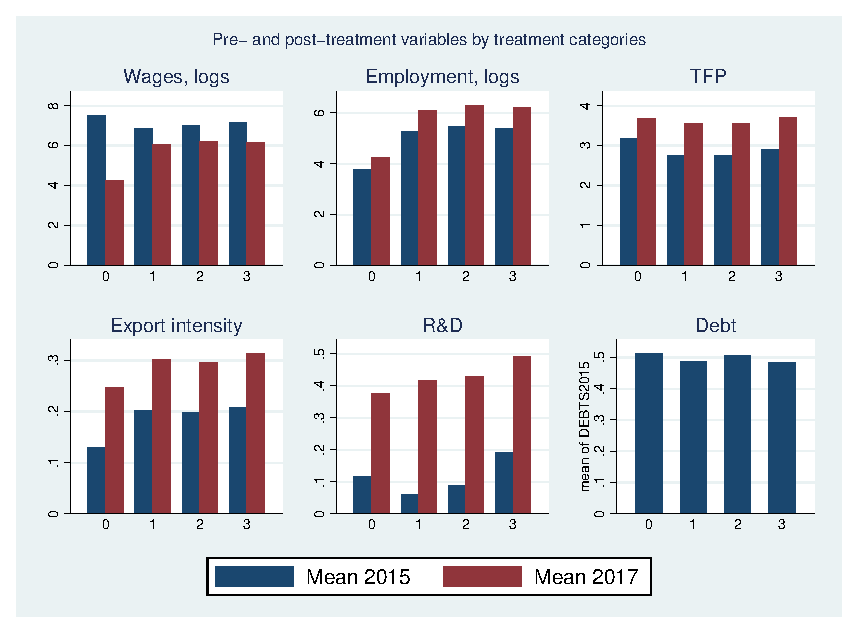
\includegraphics[scale=1]{figures/bar_pre_post} 
\end{center}
\end{figure}


\newpage

\section{Appendix}
\begin{table}[htbp]\centering 
\caption{Summary statistics for pre-treatment variables by treatment categories\label{sumstat_treatment_type_pre}}
{
\def\sym#1{\ifmmode^{#1}\else\(^{#1}\)\fi}
\begin{tabular}{l*{4}{c}}
\hline\hline
                    &\multicolumn{4}{c}{}                               \\
                    &           0&          1&           2&           3\\
                     &           No FDI&          Exports-oriented&           Techn. intensive&          Dom. market\\
                    &     Mean/SD&     Mean/SD&     Mean/SD&     Mean/SD\\
\hline
Wages in 2015 (logs)&       7.529&       6.833&       7.006&       7.146\\
                    &     (3.849)&     (3.741)&     (3.814)&     (3.824)\\
Total factor productivity in 2015&       3.185&       2.747&       2.759&       2.905\\
                    &     (2.060)&     (2.030)&     (2.006)&     (1.991)\\
Employment in 2015 (logs)&       3.766&       5.274&       5.479&       5.409\\
                    &     (3.054)&     (2.759)&     (2.706)&     (2.749)\\
Export intensity in 2015&       0.131&       0.201&       0.199&       0.209\\
                    &     (0.068)&     (0.073)&     (0.076)&     (0.077)\\
Debt in 2015 (logs) &       0.511&       0.488&       0.505&       0.485\\
                    &     (0.349)&     (0.353)&     (0.367)&     (0.352)\\
RD in 2015 (dummy)  &       0.117&       0.061&       0.089&       0.191\\
                    &     (0.321)&     (0.239)&     (0.285)&     (0.393)\\
\hline
Observations        &       6863&     940       &    1555        &    1965        \\
\hline\hline
\end{tabular}
}

\end{table} 


\begin{table}[htbp]\centering \caption{Summary statistics for post-treatment variables by treatment categories\label{sumstat_treatment_type_post}}
{
\def\sym#1{\ifmmode^{#1}\else\(^{#1}\)\fi}
\begin{tabular}{l*{4}{c}}
\hline\hline
                    &\multicolumn{4}{c}{}                               \\
                    &           1&           2&           3&           4\\
                    &     Mean/SD&     Mean/SD&     Mean/SD&     Mean/SD\\
\hline
Wages in 2017 (logs)&       4.271&       6.035&       6.216&       6.147\\
                    &     (3.063)&     (2.766)&     (2.712)&     (2.768)\\
Total factor productivity in 2017&       3.683&       3.548&       3.543&       3.703\\
                    &     (2.073)&     (2.053)&     (2.033)&     (2.014)\\
Emplyoment in 2017 (logs)&       4.265&       6.078&       6.289&       6.206\\
                    &     (3.066)&     (2.769)&     (2.719)&     (2.764)\\
Export intensity in 2017&       0.247&       0.303&       0.296&       0.313\\
                    &     (0.086)&     (0.125)&     (0.126)&     (0.130)\\
RD in 2017 (dummy)  &       0.377&       0.417&       0.430&       0.491\\
                    &     (0.485)&     (0.493)&     (0.495)&     (0.500)\\
\hline
Observations        &       6863&     940       &    1555        &    1965        \\
\hline\hline
\end{tabular}
}

\end{table} 

\begin{centering}
\begin{table}[htbp]\centering \caption{Characteristics of firms by FDI type received\label{treatment_type_char}}
\begin{tabular}[htbp!]{lrrrrrrrrrr}
\hline\hline
 & \multicolumn{10}{c}{\emph{Treatment by FDI type}} \\
\emph{Characteristics} & \multicolumn{2}{c}{\emph{No FDI}} & \multicolumn{2}{c}{\emph{Exports FDI}} & \multicolumn{2}{c}{\emph{Tech. FDI}} & \multicolumn{2}{c}{\emph{Domestic FDI}} & \multicolumn{2}{c}{\emph{Total}} \\
&No.&\%&No.&\%&No.&\%&No.&\%&No.&\% \\
\hline
Low-tech&1,869&27.2&530&56.4&805&51.8&990&50.4&4,194&37.0 \\
Medium low&904&13.2&150&16.0&290&18.6&341&17.4&1,685&14.9 \\
Medium high&2,432&35.4&220&23.4&381&24.5&506&25.8&3,539&31.3 \\
High-tech&1,658&24.2&40&4.3&79&5.1&128&6.5&1,905&16.8 \\
\emph{Total}&6,863&100.0&940&100.0&1,555&100.0&1,965&100.0&11,323&100.0 \\
\hline
No ports within 500km&4,988&72.7&479&51.0&871&56.0&1,028&52.3&7,366&65.1 \\
Ports within 500km &1,875&27.3&461&49.0&684&44.0&937&47.7&3,957&34.9 \\
\emph{Total}&6,863&100.0&940&100.0&1,555&100.0&1,965&100.0&11,323&100.0 \\
\hline
 Listed companies&736&10.7&30&3.2&63&4.1&80&4.1&909&8.0 \\
 Subsidiaries&1,615&23.5&233&24.8&351&22.6&431&21.9&2,630&23.2 \\
 Independent&2,702&39.4&403&42.9&636&40.9&852&43.4&4,593&40.6 \\
 State&1,810&26.4&274&29.1&505&32.5&602&30.6&3,191&28.2 \\
\emph{Total}&6,863&100.0&940&100.0&1,555&100.0&1,965&100.0&11,323&100.0 \\
\hline\hline
\end{tabular} 
 \end{table}
 \end{centering}


\end{document}
